%!TEX root=../GaugeCNNTheory.tex


\subsubsection*{Global rotation equivariance on $\fakebold{\Euc}_{\boldsymbol{2}} \fakebold{\backslash} \bm{\{0\}}$}
\label{sec:polar_Euc2_rot}

We start with the conceptually simplest models, which are globally rotation equivariant networks that rely on solely rotation invariant $\{e\}$-structures on~$\Euc_2 \backslash \{0\}$~\cite{finzi2020generalizing,chidester2019rotation}.
These models assume the standard Euclidean metric on~$\Euc_2 \backslash \{0\}$, relative to which the frames are orthonormal.
Together, these two requirements imply $\{e\}$-structures as shown in Fig.~\ref{fig:G_structures_R2_no_origin}.

In addition to the considered $G$-structures, the networks depend on the specific implementation of the transporter pullback and thus on the geodesics and parallel transporters.
The geodesics are in both models assumed to be the standard geodesics on Euclidean spaces (i.e. straight lines), corresponding to the Levi-Civita connection of the Euclidean metric.
As $\Euc_2 \backslash \{0\}$ is not geodesically complete, zero-padding has to be used for exponential maps that would end at the origin.
Note that this does not have an impact on the final result as the lost geodesics are of measure zero.


The parallel transport of feature vectors, on the other hand, does \emph{not} correspond to the Levi-Civita connection since the Levi-Civita connection is not compatible with the $\{e\}$-structures.
Instead, the models assume the unique $\{e\}$-compatible \emph{trivial connections} which are implied by the respective $\{e\}$-structures.%
\footnote{
\label{footnote:punctured_Euclidean_transport}
    An animation of the $\{e\}$-compatible transport corresponding to Fig.~\ref{fig:G_structure_R2_no_origin_SO2} can be found on
    \href{https://en.wikipedia.org/wiki/Levi-Civita_connection\#Parallel_transport}{\underline{Wikipedia}}.
}
According to the trivial connections, the numerical coefficients of feature vectors do not transform when being transported, despite the frames being rotated relative to the usual notion of parallelism on Euclidean spaces.
In practice, this just means that the transporters $\rho(g^{A\widetilde{A}}_\gamma) = \id_{\R^c}$ can be ignored in the implementation -- which is the reason that they are not being discussed in the original papers~\cite{finzi2020generalizing,chidester2019rotation}.


As rotations leave the considered $\{e\}$-structures invariant and are at the same time isometries, we have
$\IsomeM = \SO2$ for the model by~\citet{finzi2020generalizing} (Fig.~\ref{fig:G_structure_R2_no_origin_SO2}) and
$\IsomeM = \C8$  for the model by~\citet{chidester2019rotation} (Fig.~\ref{fig:G_structure_R2_no_origin_C8}).
Theorem~\ref{thm:isom_equiv_GM_conv} asserts then that the corresponding $\GM$-convolutions are $\IsomeM$-equivariant, which is in agreement with the statements made by the authors.

\begin{SCfigure}
    \centering
    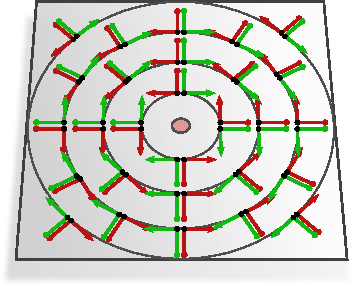
\includegraphics[width=.34\textwidth]{figures/G_structure_R2_no_origin_O2.pdf}
    \hspace*{2.ex}
    \captionsetup{width=.92\textwidth}
    \caption{\small
        An $\O2$-invariant $\Flip$-structure on $\Euc_2 \backslash \{0\}$, which is constructed by adding a reflected versions to each frame of the $\{e\}$-structure in Fig.~\ref{fig:G_structure_R2_no_origin_SO2}.
        The corresponding $\GM$-convolution is simultaneously equivariant w.r.t. global rotations and reflections in $\IsomRM = \O2$ around the origin.
        \\\protect\rule{0ex}{5.5ex}
    }
    \label{fig:G_structure_R2_no_origin_O2}
\end{SCfigure}


Before going on we want to mention that the $\C8$-invariant $\{e\}$-structure in Fig.~\ref{fig:G_structure_R2_no_origin_C8} is not continuous and does therefore not guarantee a continuous (or smooth) inference.
An advantage of this $\{e\}$-structure from an engineering viewpoint is that it is locally isometric to the canonical $\{e\}$-structure of $\R^2$, which allows to run conventional Euclidean convolution routines on each octant.
The authors discuss the generalization to $\CN$-invariant $\{e\}$-structures, which become in the limit $N\to\infty$ equivalent to the $\SO2$-invariant $\{e\}$-structure in Fig.~\ref{fig:G_structure_R2_no_origin_SO2}.

It is furthermore possible to make the models globally $\O2$-equivariant by using reflection steerable kernels instead of unconstrained kernels.
From a theoretic viewpoint this corresponds to the $\IsomRM = \O2$-invariant $\Flip$-structure $\RM$ on $\Euc_2 \backslash \{0\}$ shown in Fig.~\ref{fig:G_structure_R2_no_origin_O2}.
Note that $\RM$ is a $\Flip$-bundle over $\Euc_2 \backslash \{0\}$, whose restriction to circles of constant radius is as a principal bundle isomorphic to $\O2$, interpreted as $\Flip$-bundle over the quotient space $\O2/\Flip \cong S^1$.
